\documentclass{article}
 % Some basic packagesLLuu
\usepackage[utf8]{inputenc}
\usepackage[margin=1.2in]{geometry}
\usepackage{textcomp}
\usepackage{url}
\usepackage{graphicx}
\usepackage{float}
\usepackage{enumitem}
\usepackage{standalone}
\usepackage{tcolorbox}
\usepackage{wrapfig}
\usepackage{pgfplots} 
% \pgfplotset{compat=1.8}
% \pgfplotsset{scaled y ticks=false}
% \usepackage{svg}
% \usepackage{svg-inkscape} 

%color settings
\usepackage{xcolor}
\definecolor{gruvbgdark}{HTML}{1d2021}
\definecolor{gruvtextdark}{HTML}{ebdbb2}
\definecolor{gruvbglight}{HTML}{f9f5d7}
\definecolor{gruvtextlight}{HTML}{3c3836}
\definecolor{NavyBlue}{HTML}{266bbd}
\definecolor{RawSienna}{HTML}{94330e}
\definecolor{ForestGreen}{HTML}{149b52}
% \pagecolor{gruvbgdark}
% \color{gruvtextdark}

% Hide page number when page is empty
\usepackage{emptypage}
\usepackage{subcaption}
\usepackage{multicol}

% Math stuff
\usepackage{amsmath, amsfonts, mathtools, amsthm, amssymb}
% Fancy script capitals
\usepackage{mathrsfs}
\usepackage{cancel}

% Bold math
\usepackage{bm}

% SVG setup
% \svgsetup{inkscapeexe=inkscape, inkscapearea=drawing}
% \svgpath{~/dev/DAVE3700-Matte-3000/figures/}

% Some shortcuts
\newcommand\N{\ensuremath{\mathbb{N}}}
\newcommand\R{\ensuremath{\mathbb{R}}}
\newcommand\Z{\ensuremath{\mathbb{Z}}}
\renewcommand\O{\ensuremath{\emptyset}}
\newcommand\Q{\ensuremath{\mathbb{Q}}}
\newcommand\C{\ensuremath{\mathbb{C}}}

%Make implies and impliedby shorter
\let\implies\Rightarrow
\let\impliedby\Leftarrow
\let\iff\Leftrightarrow

\let\epsilon\varepsilon

% Add \contra symbol to denote contradiction
% \usepackage{stmaryrd} % for \lightning
% \newcommand\contra{\scalebox{1.5}{$\lightning$}}

\let\phi\varphi

% Command for short corrections
% Usage: 1+1=\correct{3}{2}

\definecolor{correct}{HTML}{009900}
\newcommand\correct[2]{\ensuremath{\:}{\color{red}{#1}}\ensuremath{\to }{\color{correct}{#2}}\ensuremath{\:}}
\newcommand\green[1]{{\color{correct}{#1}}}

% horizontal rule
% \newcommand\hr{
%     \noindent\rule[0.5ex]{\linewidth}{0.5pt}
% }

% hide parts
\newcommand\hide[1]{}

% Environments
\makeatother

% For box around Definition, Theorem, \ldots
% theorems
\usepackage{thmtools}
\usepackage[framemethod=TikZ]{mdframed}
\mdfsetup{skipabove=1em,skipbelow=1em, innertopmargin=5pt, innerbottommargin=6pt}

\theoremstyle{definition}

\makeatletter

% \declaretheoremstyle[headfont=\bfseries, bodyfont=\normalfont, mdframed={ nobreak } ]{thmgreenbox}
% \declaretheoremstyle[headfont=\bfseries, bodyfont=\normalfont, mdframed={ nobreak } ]{thmredbox}
% \declaretheoremstyle[headfont=\bfseries, bodyfont=\normalfont, spaceabove=0.5cm, spacebelow=0.5cm]{thmbluebox}
% % \declaretheoremstyle[headfont=\bfseries, bodyfont=\normalfont]{thmbluebox}
% \declaretheoremstyle[headfont=\bfseries, bodyfont=\normalfont]{thmblueline}
% \declaretheoremstyle[headfont=\bfseries, bodyfont=\normalfont, numbered=no, mdframed={ rightline=false, topline=false, bottomline=false, }, qed=\qedsymbol ]{thmproofbox}
% \declaretheoremstyle[headfont=\bfseries\sffamily, bodyfont=\normalfont, numbered=no, mdframed={ nobreak, rightline=false, topline=false, bottomline=false } ]{thmexplanationbox}
\declaretheoremstyle[headfont=\bfseries, bodyfont=\normalfont, numbered=no]{idea}

\declaretheoremstyle[
	headfont=\bfseries\color{ForestGreen!70!black}, bodyfont=\normalfont,
	mdframed={
			linewidth=2pt,
			rightline=false, topline=false, bottomline=false,
			linecolor=ForestGreen, backgroundcolor=ForestGreen!5,
		}
]{thmgreenbox}

\declaretheoremstyle[
	headfont=\bfseries\color{NavyBlue!70!black}, bodyfont=\normalfont,
	mdframed={
			linewidth=2pt,
			rightline=false, topline=false, bottomline=false,
			linecolor=NavyBlue, backgroundcolor=NavyBlue!5,
		}
]{thmbluebox}

\declaretheoremstyle[
	headfont=\bfseries\color{NavyBlue!70!black}, bodyfont=\normalfont,
	mdframed={
			linewidth=2pt,
			rightline=false, topline=false, bottomline=false,
			linecolor=NavyBlue
		}
]{thmblueline}

\declaretheoremstyle[
	headfont=\bfseries\color{RawSienna!70!black}, bodyfont=\normalfont,
	mdframed={
			linewidth=2pt,
			rightline=false, topline=false, bottomline=false,
			linecolor=RawSienna, backgroundcolor=RawSienna!5,
		}
]{thmredbox}

\declaretheoremstyle[
	headfont=\bfseries\color{RawSienna!70!black}, bodyfont=\normalfont,
	numbered=no,
	mdframed={
			linewidth=2pt,
			rightline=false, topline=false, bottomline=false,
			linecolor=RawSienna, backgroundcolor=RawSienna!0,
		},
	qed=\qedsymbol
]{thmproofbox}

\declaretheoremstyle[
	headfont=\bfseries\color{NavyBlue!70!black}, bodyfont=\normalfont,
	numbered=no,
	mdframed={
			linewidth=2pt,
			rightline=false, topline=false, bottomline=false,
			linecolor=NavyBlue, backgroundcolor=NavyBlue!1,
		},
]{thmexplanationbox}

\declaretheorem[style=thmgreenbox, name=Definisjon]{definition}
\declaretheorem[sibling=definition, style=thmredbox, name=Corollary]{corollary}
\declaretheorem[style=idea, name=Idea]{idea}
\declaretheorem[style=idea, style=thmredbox, name=Proposition]{prop}
\declaretheorem[sibling=definition, style=thmredbox, name=Theorem]{theorem}
\declaretheorem[sibling=definition, style=thmredbox, name=Lemma]{lemma}



\declaretheorem[numbered=no, style=thmexplanationbox, name=Proof]{explanation}
\declaretheorem[numbered=no, style=thmproofbox, name=Proof]{replacementproof}
\declaretheorem[style=thmbluebox,  numbered=no, name=Exercise]{ex}
\declaretheorem[style=thmbluebox,  numbered=no, name=Svar]{ans}
\declaretheorem[style=thmbluebox,  numbered=no, name=Example]{eg}
\declaretheorem[style=thmblueline, numbered=no, name=Remark]{remark}
\declaretheorem[style=thmblueline, numbered=no, name=Note]{note}

\renewenvironment{proof}[1][\proofname]{\begin{replacementproof}}{\end{replacementproof}}

\AtEndEnvironment{eg}{\null\hfill$\diamond$}%

\newtheorem*{uovt}{UOVT}
\newtheorem*{notation}{Notation}
\newtheorem*{previouslyseen}{As previously seen}
\newtheorem*{problem}{Problem}
\newtheorem*{observe}{Observe}
\newtheorem*{property}{Property}
\newtheorem*{intuition}{Intuition}


% Exercise 
% Usage:
% \oefening{5}
% \suboefening{1}
% \suboefening{2}
% \suboefening{3}
% gives
% Oefening 5
%   Oefening 5.1
%   Oefening 5.2
%   Oefening 5.3
\newcommand{\oefening}[1]{%
	\def\@oefening{#1}%
	\subsection*{Oefening #1}
}

\newcommand{\suboefening}[1]{%
	\subsubsection*{Oefening \@oefening.#1}
}


% \lecture starts a new lecture (les in dutch)
%
% Usage:
% \lecture{1}{di 12 feb 2019 16:00}{Inleiding}
%
% This adds a section heading with the number / title of the lecture and a
% margin paragraph with the date.

% I use \dateparts here to hide the year (2019). This way, I can easily parse
% the date of each lecture unambiguously while still having a human-friendly
% short format printed to the pdf.

% \usepackage{xifthen}
% \def\testdateparts#1{\dateparts#1\relax}
% \def\dateparts#1 #2 #3 #4 #5\relax{
% 	\marginpar{\small\textsf{\mbox{#1 #2 #3 #5}}}
% }

% \def\@lecture{}%
% \newcommand{\lecture}[3]{
% 	\ifthenelse{\isempty{#3}}{%
% 		\def\@lecture{Lecture #1}%
% 	}{%
% 		\def\@lecture{Lecture #1: #3}%
% 	}%
% 	\subsection*{\@lecture}
% 	% \marginpar{\small\textsf{\mbox{#2}}}
% }

\usepackage{listings}
\usepackage{color}

\definecolor{dkgreen}{rgb}{0,0.6,0}
\definecolor{gray}{rgb}{0.5,0.5,0.5}
\definecolor{mauve}{rgb}{0.58,0,0.82}

\lstset{frame=tb,
  language=Java,
  aboveskip=3mm,
  belowskip=3mm,
  showstringspaces=false,
  columns=flexible,
  basicstyle={\small\ttfamily},
  numbers=none,
  numberstyle=\tiny\color{gray},
  keywordstyle=\color{blue},
  commentstyle=\color{dkgreen},
  stringstyle=\color{mauve},
  breaklines=true,
  breakatwhitespace=true,
  tabsize=3
}


% These are the fancy headers
\usepackage{fancyhdr}
\pagestyle{fancy}

% LE: left even
% RO: right odd
% CE, CO: center even, center odd
% My name for when I print my lecture notes to use for an open book exam.
\fancyhead[LE,RO]{Kristian Sørdal}

\fancyhead[RO,LE]{INF102 - Algoritmer og Data Strukturer} % Right odd,  Left even
\fancyhead[RE,LO]{\leftmark}          % Right even, Left odd

\fancyfoot[RO,LE]{\thepage}  % Right odd,  Left even
\fancyfoot[RE,LO]{}          % Right even, Left odd
\fancyfoot[C]{\leftmark}     % Center

\makeatother

% Todonotes and inline notes in fancy boxes
\usepackage{todonotes}
\usepackage{tcolorbox}

% Make boxes breakable
\tcbuselibrary{breakable}

% Figure support as explained in my blog post.
\usepackage{import}
\usepackage{xifthen}
\usepackage{pdfpages}
\usepackage{transparent}
\newcommand{\incfig}[2][1]{%
	% \begin{center}
	\def\svgwidth{#1\columnwidth}
	\import{./figures/}{#2.pdf_tex}
	% \end{center}
}

\graphicspath{{./figures/}}
% Fix some stuff
% %http://tex.stackexchange.com/questions/76273/multiple-pdfs-with-page-group-included-in-a-single-page-warning
\pdfsuppresswarningpagegroup=1
\author{Kristian Sørdal}

\begin{document}
   \section{Week 1} 
   \subsection{Task 1}

Given a list of integers, write an algorithm that selects the three numbers that summed gives the largest value. 
\( [8, 19, -1, 27, 3, 9, -40] \). The largest value that three of the numbers sums to is 55. What runtime does your algorithm have?

\subsubsection{Solution}
I came up with two solutions for this problem, the first problem is a rather slow solution, and as there are three nested for loops, this program runs in \( O\left( n^3 \right) \) time.

\begin{figure}[H]
    \begin{center}
        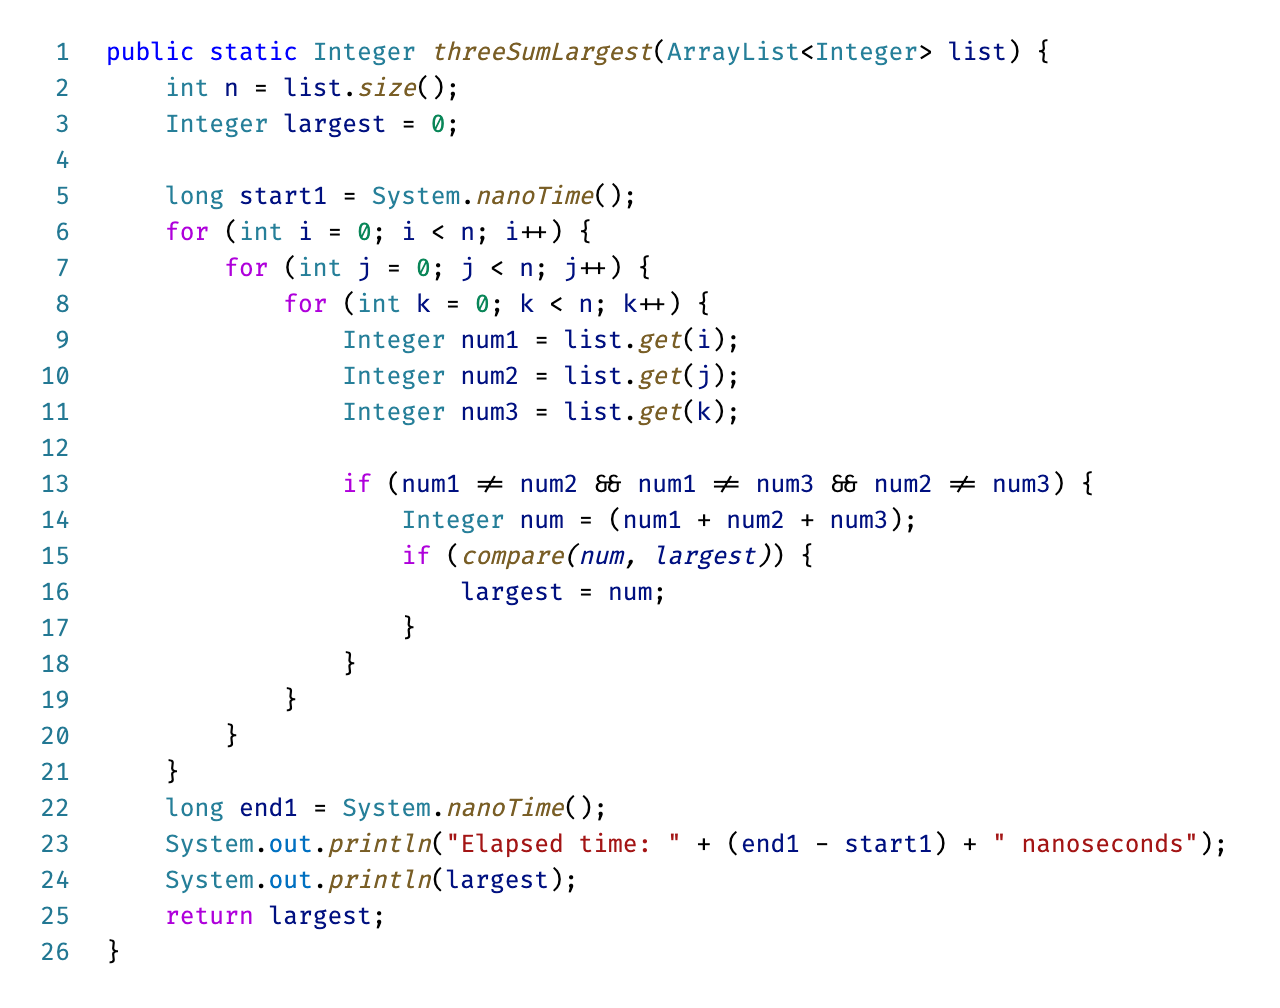
\includegraphics[width=0.95\textwidth]{threeSumLargest.png}
    \end{center}
    \caption{First solution for this problem}
    \label{fig:threeSumLargest}
\end{figure}

The second solution is slightly faster, however finding its time complexity is slightly harder, as we are using some methods from the \textit{Collections} framework. As shown in Figure \ref{fig:fastThreeSumLargest.png}, we can see that \textit{Collections.Sort} and has been used. Doing a quick google search, we find that this method has a time complexity of \( O\left( n \log\left( n \right) \right) \).

\begin{figure}[H]
    \begin{center}
        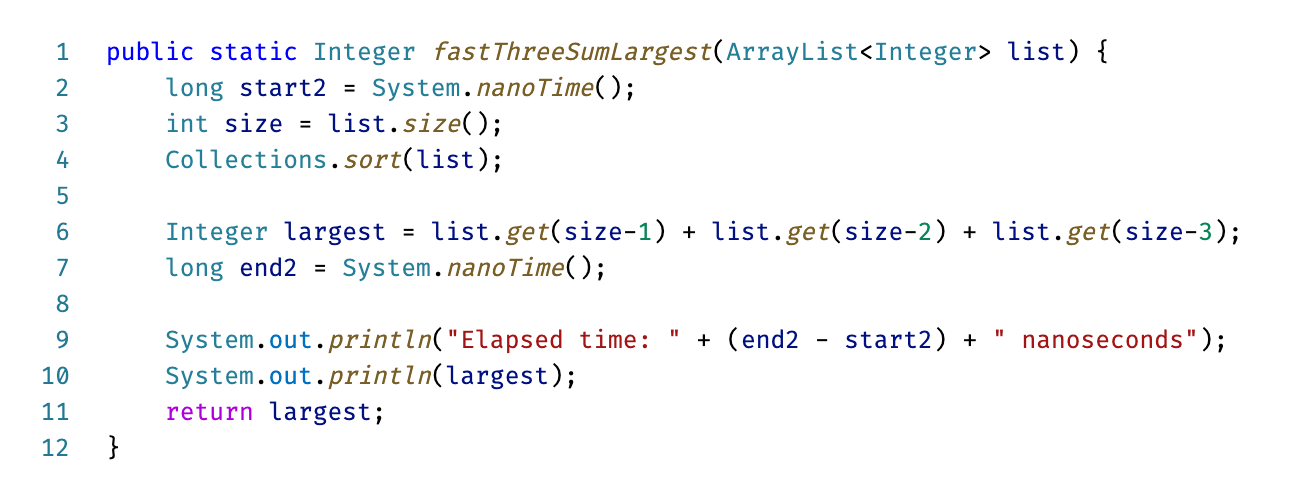
\includegraphics[width=0.95\textwidth]{fastThreeSumLargest.png}
    \end{center}
    \caption{Second solution, slightly faster}
    \label{fig:fastThreeSumLargest.png}
\end{figure}

Comparing the two solutions, we get the the following graph. As we can see, the faster solution is vastly surperior to the slower version.

\begin{center}
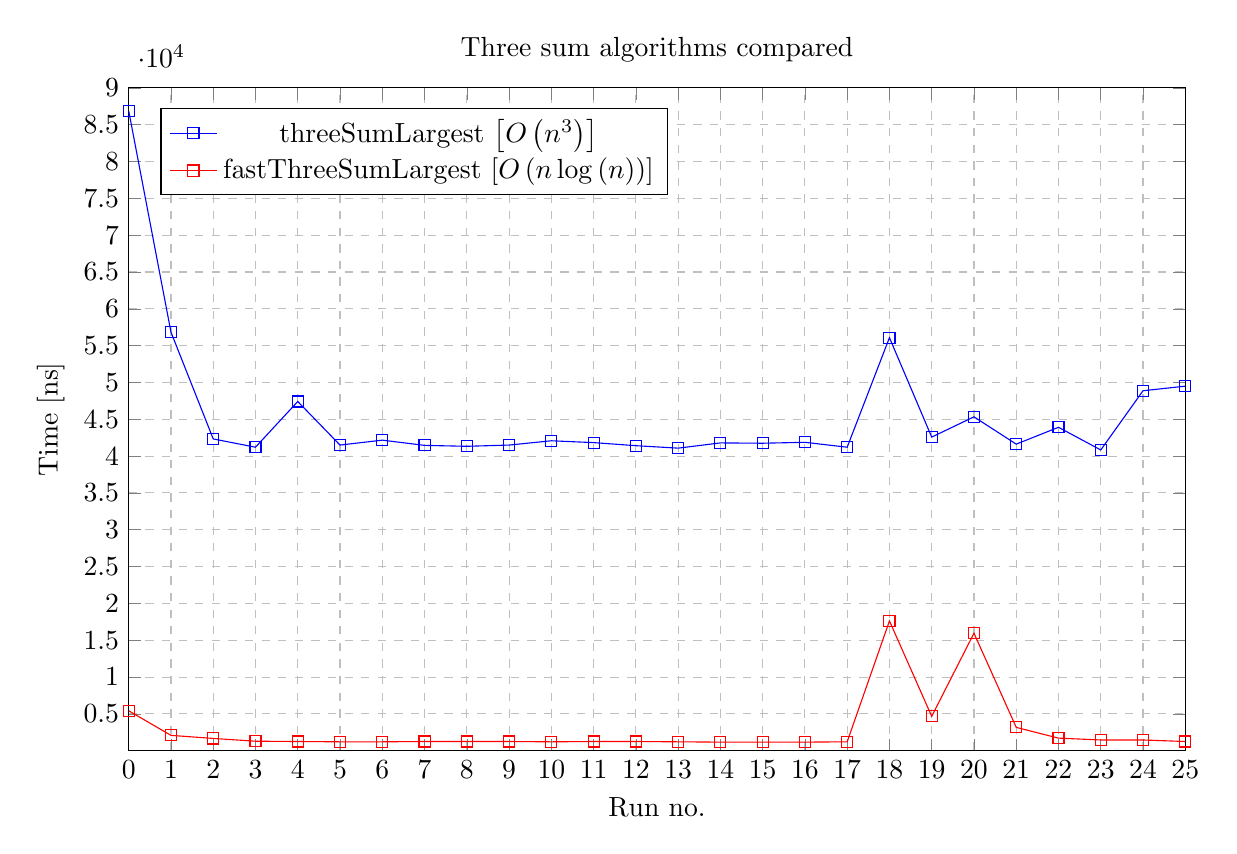
\begin{tikzpicture}
\begin{axis}[
    title={Three sum algorithms compared},
    xlabel={Run no.},
    ylabel={Time [ns]},
    xmin=0, xmax=25,
    ymin=0, ymax=90000,
    xtick={0,1,...,25},
    ytick={5000,10000,...,90000},
    legend pos=north west,
    ymajorgrids=true,
    xmajorgrids=true,
    grid style=dashed,
    width = 15cm,
    height = 10cm,
]

\addplot[
    color=blue,
    mark=square,
    ]
    coordinates {
    (0,86875)(1,56833)(2,42333)(3,41209)(4,47417)(5,41500)(6,42167)(7,41458)(8,41333)(9,41500)(10,42083)(11,41833)(12,41416)(13,41083)(14,41792)(15,41750)(16,41875)(17,41208)(18,56083)(19,42583)(20,45333)(21,41625)(22,43917)(23,40834)(24,48875)(25,49500)
    };
    % \legend{threeSumLargest}

\addplot[
    color=red,
    mark=square,
    ]
    coordinates {
(0,5417)(1,2084)(2,1667)(3,1291)(4,1250)(5,1209)(6,1209)(7,1250)(8,1250)(9,1250)(10,1208)(11,1250)(12,1250)(13,1208)(14,1166)(15,1167)(16,1167)(17,1208)(18,17625)(19,4667)(20,15958)(21,3166)(22,1709)(23,1458)(24,1458)(25,1250)
    };
\legend{threeSumLargest \(  \left[ O\left( n^3 \right) \right] \), fastThreeSumLargest \( \left[ O\left( n \log\left( n \right) \right) \right] \)}
    
\end{axis}
\end{tikzpicture}
\end{center}

\subsection{Task 2}
Given a sorted list of integers, write an algorithm that runs in linear time \( (O(n)) \) that determines if two numbers sum to 0.  \( [-10, -8, -4, -1, 5, 8, 18, 20, 40] \). mk and \( 8 \) sum to \( 0 \) hence this list should yield \textit{true}.

\subsubsection{Solution}
This problem is a \textit{two sum} problem, which usually is solved with a time complexity of \( O\left( n^2 \right) \). Again two solutions were developed, one of which is the standard solution, running in \( O\left( n^2 \right) \) time, and the other being a faster solution, running in \( O\left( n \right) \) time, or linear time.
\bigskip

The first solution uses two nested for loops to check if two of the integers sum to the desired goal sum. Because there are two for loops, its a rather slow solution, and it runs in \( O\left( n^2 \right) \) time, as mentioned.

\begin{figure}[H]
    \begin{center}
        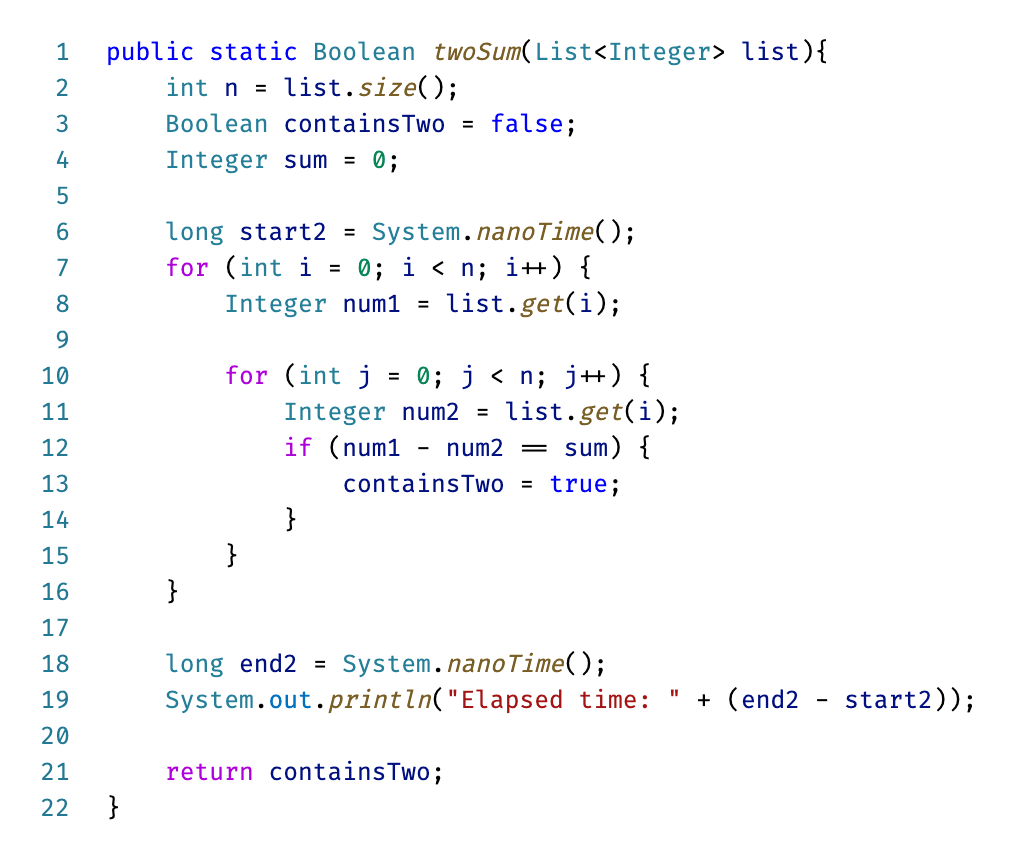
\includegraphics[width=0.95\textwidth]{twoSum.png}
    \end{center}
    \caption{First and slower solution of the problem}
    \label{fig:twoSum.png}
\end{figure}

The faster solutions, employs the usage of an empty HashSet. It then loops through the list and checks if one of three conditions are met. The first condition occurs when the set is empty, is the simply adds the currenet element to the list. Next it checks if the set \textit{doesn't} contain the result of the sum subtracted from the current element, if it doesn't, it adds the current element to the list. Lastly, if none of the previous conditions are met, it means that we have found that two integers in the list sum to our desired sum, and the variable \textit{containsTwo} is set to true.

\begin{figure}[H]
    \begin{center}
        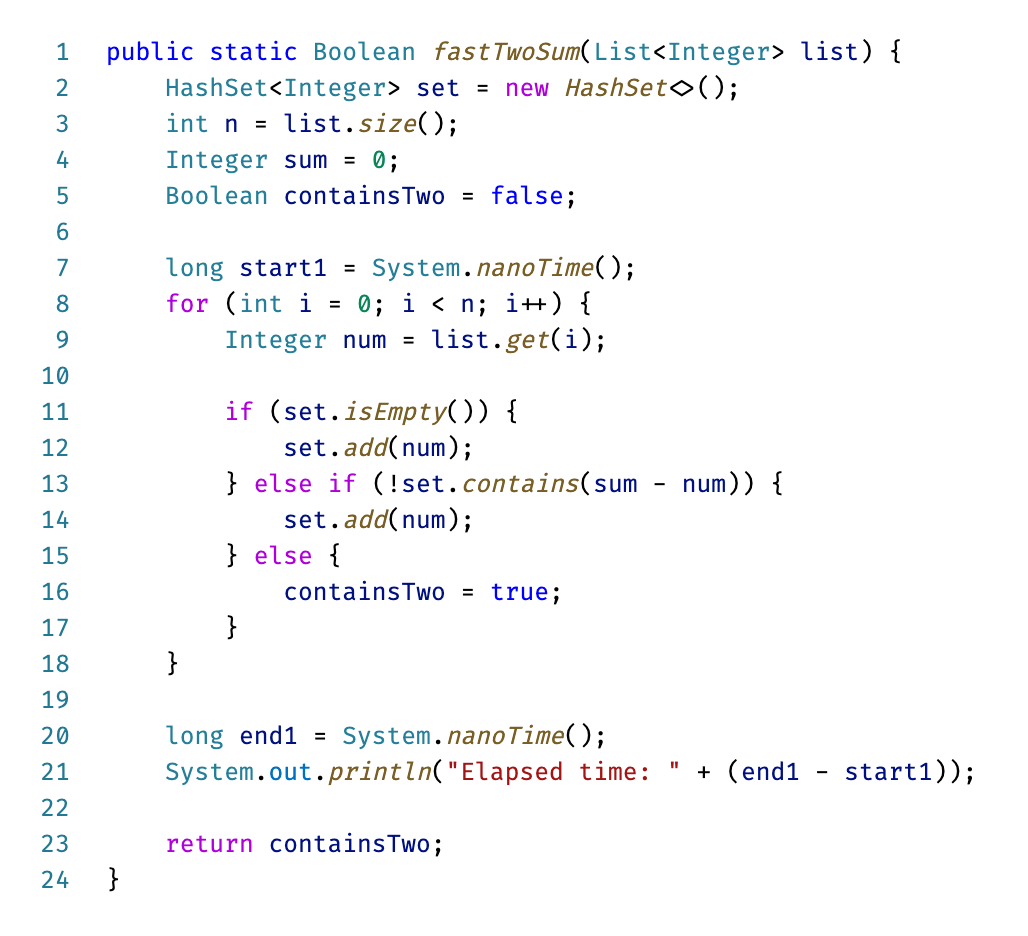
\includegraphics[width=0.95\textwidth]{fastTwoSum.png}
    \end{center}
    \caption{Second, faster solution}
    \label{fig:fastTwoSum.png}
\end{figure}

\begin{center}
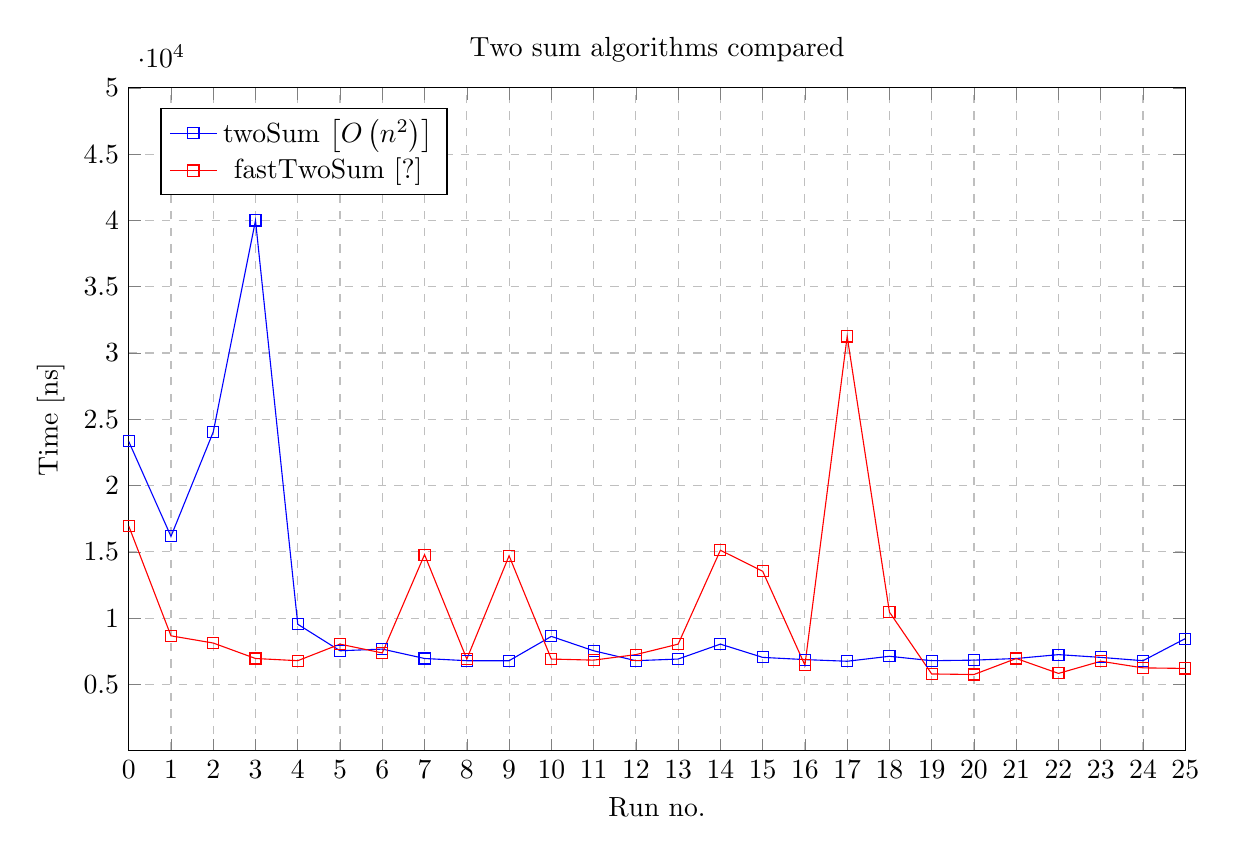
\begin{tikzpicture}
\begin{axis}[
    title={Two sum algorithms compared},
    xlabel={Run no.},
    ylabel={Time [ns]},
    xmin=0, xmax=25,
    ymin=0, ymax=50000,
    xtick={0,1,...,25},
    ytick={5000,10000,...,90000},
    legend pos=north west,
    ymajorgrids=true,
    xmajorgrids=true,
    grid style=dashed,
    width = 15cm,
    height = 10cm,
]

\addplot[
    color=blue,
    mark=square,
    ]
    coordinates {
    (0,23333)(1,16167)(2,24041)(3,40000)(4,9542)(5,7541)(6,7667)(7,6958)(8,6792)(9,6791)(10,8625)(11,7541)(12,6792)(13,6917)(14,8042)(15,7042)(16,6875)(17,6750)(18,7125)(19,6792)(20,6833)(21,6958)(22,7250)(23,7042)(24,6792)(25,8459)
    };
    % \legend{threeSumLargest}

\addplot[
    color=red,
    mark=square,
    ]
    coordinates {
    (0,16959)(1,8667)(2,8125)(3,6958)(4,6792)(5,8041)(6,7375)(7,14791)(8,6917)(9,14708)(10,6917)(11,6834)(12,7250)(13,8042)(14,15125)(15,13542)(16,6458)(17,31250)(18,10459)(19,5792)(20,5750)(21,6958)(22,5833)(23,6750)(24,6250)(25,6209)
    };
    \legend{twoSum \( \left[ O\left( n^2 \right) \right] \), fastTwoSum \( \left[ ? \right] \)}
    
\end{axis}
\end{tikzpicture}
\end{center}

As we can see, it does not look like the "faster" version of this algorithm actually is faster, further optimization is certainly appropriate.

\subsection{Task 3}
Sort the functions based on which grows fastest when n becomes large:

\begin{itemize}
\item \(f(n)\) = \( n^2 + n \)
\item \(f(n)\) = \( n * \log (n) \)
\item \(f(n)\) = \( n \cdot  n \)
\item \(f(n)\) = \( n \cdot  (log(n))^3 \)
\end{itemize}
\newpage 

The functions above grow fastest according to the following list

\begin{enumerate}
    \item \(f(n)\) = \( n^2 + n \)
    \item \(f(n)\) = \( n \cdot  n \)
    \item \(f(n)\) = \( n \cdot  (log(n))^3 \)
    \item \(f(n)\) = \( n * \log (n) \)
\end{enumerate}



\end{document}
